\documentclass[11pt]{article}

\usepackage[utf8]{inputenc}
%%\usepackage[T1]{fontenc}
\usepackage{graphicx}
\usepackage[linktocpage=true]{hyperref}

%%Page layout
\usepackage[margin=2.0cm]{geometry}
\usepackage{bookmark}

%%Figures
\usepackage{float}

\usepackage{mathpazo}

%%Font and Numbers
\renewcommand*\rmdefault{dayrom}
\usepackage[T1]{fontenc}
\normalfont
\usepackage{enumitem}

%%Packages for Referrences
\usepackage{url}
\usepackage{etoolbox}
\patchcmd{\thebibliography}{\section*{\refname}}{}{}{}
\patchcmd{\thebibliography}{\addcontentsline{toc}{section}{\refname}}{}{}{}

%%Group Comments
\usepackage{verbatim}

\usepackage{titlesec}

\setcounter{secnumdepth}{4}

\titleformat{\paragraph}
{\normalfont\normalsize\bfseries}{\theparagraph}{1em}{}
\titlespacing*{\paragraph}
{0pt}{3.25ex plus 1ex minus .2ex}{1.5ex plus .2ex}

\begin{document}
\renewcommand{\familydefault}{\sfdefault}
\begin{titlepage}
	\newcommand{\HRule}{\rule{\linewidth}{0.5mm}}
	\begin{center}
		            
		\textsc{\LARGE Alabama Liquid Snake}\\[0.8cm]
		\textsc{\Large University of Pretoria}\\[0.5cm]
		\textsc{\large Epi-Use}\\[0.5cm]
		    
		\HRule\\[0.4cm]
		    	
		{\huge\bfseries Botic - Privacy aware chatbot}\\[0.2cm]
		    	
		{\huge Process and Methodology}\\[0.2cm]
		
		\HRule\\[0.5cm]
		
		\textsc{Justin Grenfell} - u16028440 \\[0cm]
		\textsc{Peter Msimanga} - u13042352 \\[0cm]
		\textsc{Alicia Mulder} - u14283124 \\[0cm]
		\textsc{Kyle Gaunt} - u15330967 \\[0cm]
		\textsc{Lesego Mabe} - u15055214 \\[0cm]
		    
	\end{center}
\end{titlepage}
\tableofcontents
\newpage

\section{Introduction}
\subsection{Agile Unified Methodology}

<Provide a Diagram of the AUM>

Using the Agile Unified Methodology to take advantage of agile principles as well as work with a methodology based off the
waterfall process, that has a simple linear and uncomplicated progression is what we have chosen to do. We anticipate that
the project will not have a high requirements change throughout development, and this makes the waterfall process derivative
methodology more fitting.

The Agile Unified Methodology makes use of Test-Driven Development, which makes it easier to develop high quality code.
<Provide details of how we would deal with the set backs of the Test-Driven Development>
<Additional motivations>

At the moment, phase 3 has high priority.

\section{Planning Phase}

\subsection{Acquiring Requirements}

\subsubsection{Specific Functional Requirements and Constraints}

\paragraph{User Interface}
\begin{itemize}
  \item[] R1.1 The system must allow a customer to enter a query and click on a button to send it.
  \item[] R1.2 The system must warn a customer of personal information included in a query.
  \item[] R2.2 The system must be able to highlight personally identifying information according to severity index.
  \item[] R3.3.2.2 The system must be able to highlight personally identifying information according to severity index.
  \item[] R3.3.2.3 The system must be able to warn the client representative if they have entered identifying information.
  \item[] R4.1 The system must allow customers to thumbs up a query response.
  \item[] R4.2 The system must allow customers to thumbs down a query response.
  \item[] R5 The system must allow queries to be sent to customer support representatives if not answered satisfactorily.
  \item[] C1 The system must use an Angular Single Page Application for the user interface.
\end{itemize}

\paragraph{Information Scraper}
\begin{itemize}
  \item[] R2.1 The system must be able to attach a severity to the personally identifying information.
  \item[] R3.1 The system must scrape its customer query responses for personal information.
  \item[] R3.3.2.1 The system must be able to identify personal information in a customer representative's response. 
  \item[] C3.1 The system must use word2vec for identifying personal information in customer queries.
  \item[] C5.2 The system must determine if the response contains personally identifying information.
\end{itemize}

\paragraph{Query Classification}
\begin{itemize}
  \item[] R3.2 The system must be able to classify the user queries.
  \item[] C3.2 The system must use word2vec for classifying customer queries.
\end{itemize}

\paragraph{Response Generation}
\begin{itemize}
  \item[] R3.3.1 The system must generate a response if it certain that it can.
  \item[] C5.1 The system must generate an automated response based on the query classification.
\end{itemize}

\paragraph{Chatbot}
\begin{itemize}
  \item[] R1.3 The system must be able to recieve customer queries.
  \item[] R3.3.2 The system must be able to send the query to a customer support representative if it cannot obtain an appropriate response.
  \item[] R3.4 The system must be able to send a query response back to a customer.
  \item[] R4.3 The system must be able to recieve customer feedback.
  \item[] R5 The system must allow queries to be sent to customer support representatives if not answered satisfactorily.
  \item[] R8 The system must interface with the currently existing ticket system.
  \item[] C2 The system must provide an API for the SPA to interact with.
\end{itemize}

\paragraph{Chatbot Trainer}
\begin{itemize}
  \item[] R6.1 The system must store previous customer interactions with positive feedback.
  \item[] R7 The system must must be trained with previous customer queries and responses.
  \item[] C4 The system must use Machine Learning or Deep Neural Networks in order to be trained with previous customer queries and responses.
\end{itemize}

\paragraph{Data Persistence}
\begin{itemize}
  \item[] R9.1 The system must scrape customer interation data for personal information before storing.
\end{itemize}

\subsubsection{Functional Clusters and Functional Subsystems}
\begin{center}
	\hspace*{-1.5cm}\begin{tabular}{|p{4cm}|p{7cm}|p{3cm}|p{5cm}|}
		\hline
		Functional Cluster & Functional Description & System Requirements & Function Subsystem Identified \\
		\hline
		User Interface & This functional cluster allows customers and customer support representatives to interact with the system & R1.1, R1.2, R2.2, R3.3.2.2, R3.3.2.3, R4.1, R4.2, R5, C1 & User Interface Subsystem \\
		\hline 
		Personal Information Identification & This functional cluster identifies personal information within messages & R2.1, R3.1, R3.3.2.1, C3.1, C5.2 & Message Scraper Subsystem \\
		\hline
		Classification of Queries & This functional cluster is responsible for classifying queries. & R3.2, C3.2 & Query Classification Subsystem \\
		\hline
		Automatic Query Response Generation & This functional cluster is responsible for generating query responses & R3.3.1, C5.1 & Response Generation Subsystem \\
		\hline
		Main Program & This function cluster is responsible for coordinating query handling subsystems & R1.3, R3.3.2, R3.4, R4.3, R5, R8, C2 & Chatbot Subsystem \\
		\hline
		ChatBot Training & This functional cluster is responsible for training the system using previous interactions & R6.1, R7, C4 & Chatbot Trainer Subsystem \\
		\hline
		 Data Persistence & This functional cluster is responsible for persisting customer interactions & R9.1 & Database Subsystem \\
		\hline
	\end{tabular}
\end{center}

\subsubsection{Traceability Matrix}
\begin{center}
	\hspace*{-1.3cm}\begin{tabular}{|c|c|c|c|c|c|c|c|}
	\hline
	R & UI & Info Scraper & Query Classification & Resp Generation & Chatbot & Chatbot Trainer & Data Persistence \\
	\hline
	R1.1 & X & & & & & & \\
	\hline
	R1.2 & X & & & & & & \\
	\hline
	R1.3 & & & & X & & & \\
	\hline
	R2.1 & & X & & & & & \\
	\hline
	R2.2 & X & & & & & & \\
	\hline
	R3.1 & & X & & & & & \\
	\hline
	R3.2 & & & X & & & & \\
	\hline
	R3.3.1 & & & & X & & & \\
	\hline
	R3.3.2 & & & & & X & & \\
	\hline
	R3.3.2.1 & & X & & & & & \\
	\hline
	R3.3.2.2 & X & & & & & & \\
	\hline
	R3.3.2.3 & X & & & & & & \\
	\hline
	R3.4 & & & & & X & & \\
	\hline
	R4.1 & X & & & & & & \\
	\hline
	R4.2 & X & & & & & & \\
	\hline
	R4.3 & X & & & & & & \\
	\hline
	R5 & X & & & & X & & \\
	\hline
	R6.1 & & & & & & X & \\
	\hline
	R7 & & & & & & X & \\
	\hline
	R8 & & & & & X & & \\
	\hline
	R9.1 & & & & & & & X \\
	\hline
	C1 & X & & & & & & \\
	\hline
	C2 & & & & & X & & \\
	\hline
	C3.1 & X & & & & & & \\
	\hline
	C3.2 & & & X & & & & \\
	\hline
	C4 & & & & & & X & \\
	\hline
	C5.1 & & & & X & & & \\
	\hline
	C5.2 & & X & & & & & \\
	\hline
	\end{tabular}
\end{center}

Key: UI = User Interface, Info Scraper = Information Scraper, Resp Generation =  Response Generation.

\subsubsection{Nonfunctional Requirements/Quality Attributes}

\paragraph{Security Requirements}
\begin{enumerate}[label=R1.\arabic*.]
	\item The system must be able to authenticate users and authorize them to access system features.
	\begin{enumerate}[label*=\arabic*.]
		\item The system must be able to identify and authenticate customers.
		\item The system must be able to identify and authenticate customer support representatives.
		\item The system must be able to deny users who haven't been authenticated to access system features
	\end{enumerate}
	\item The system must be able to allow new users to register for user profiles for authentication.
	\item The system must be able to allow users to update their password.
	\item The system must ensure that confidentiality of customer and customer support representative interactions are ensured and maintained across the system.
	\begin{enumerate}[label*=\arabic*.]
		\item The system must ensure that customers can interact with the system in a secured manner.
		\item The system must ensure that customer queries are sent in a secured manner.
		\item The system must ensure that customer support representatives care interact with the system in a secured manner.
		\item The system must ensure that customer support representative response are sent in a secured manner.
		\item The system must ensure that all queries and responses are processed in a secured manner.
	\end{enumerate}
	\item The system must ensure that information disclosed during error management is not revealing of internal architecture, design, and configuration information.
\end{enumerate}

\paragraph{Availability}
\begin{enumerate}[label=R1.\arabic*.]
	\item The system must have high availability to handle customer queries.
	\begin{enumerate}[label*=\arabic*.]
		\item The system should be available at least 99 percent of the time.
	\end{enumerate}
	\item The system must ensure that errors that occur throughout the system are handled appropriately and provide sufficient
information.
	\begin{enumerate}[label*=\arabic*.]
		\item The system must provide error messages when errors occur.
		\item The system must ensure to keep a traces that show what led to errors.
	\end{enumerate}
	\item The system must ensure that errors are localized and that their effect is minimized throughout the system.
\end{enumerate}

\paragraph{Reliability}
\begin{enumerate}[label=R1.\arabic*.]
	\item The system must ensure that responses to customer queries are done in a reliable manner.
	\begin{enumerate}[label*=\arabic*.]
		\item The system must ensure that customer support representative are authorized to respond to customer queries.
		\item The system must ensure that queries are responses sent throughout the system are complete and consistent.
	\end{enumerate}
	\item The system must ensure that it is at least 80 percent certain that an autogenerated response is correct before responding to a query.
\end{enumerate}

\paragraph{Performance}
\begin{enumerate}[label=R1.\arabic*.]
	\item The system must ensure that personal information is highlighted according to severity in real-time.
	\begin{enumerate}[label*=\arabic*.]
		\item The system must ensure that a severity of a word is recieved within a second of it being typed.
		\item The system must ensure that a word or set of words containing personal information are highlighted in less than a second after recieving the severity.
	\end{enumerate}
\end{enumerate}

%Should be made testable
\paragraph{Maintainability}
\begin{enumerate}[label=R1.\arabic*.]
	\item The system must allow for system changes and modifications to the user interface to be made as seemlessly as possible.
	\item The system must allow for system changes to the database to be made as seemlessly as possible.
\end{enumerate}

\subsection{Deriving Use Cases from Requirements}

modeling and anaylsis of misuse cases
- role based access rights
- nonfunctional requirement associations i.e. security requirements, should be associated using the requirement-use case traceability matrix

Using the steps as defined in \cite{Book:1} page 176 to 192, namely: identifying use cases, specifying use case scopes, visualizing use case contexts, reviewing the use cases and diagrams, and finally allocating the use cases to iterations.

\subsubsection{Identifying Use Cases}

\paragraph{Deriving Use Cases, Actors, and Subsystems}
\begin{center}
	\hspace*{-0.9cm}\begin{tabular}{|p{2cm}|p{2cm}|p{2cm}|p{2cm}|p{2cm}|p{2cm}|p{2cm}|p{2cm}|}
		\hline
		Verb-Noun Phrase & Is it a business process? & Does it begin with an actor? & Does it end with the actor? & Does it accomplish a business task for the actor? & Is it a use case? & Actor & Subsystem \\
		\hline
		Startup System & Y & Y & Y & Y & Y & Admin & Botic \\
		\hline
		Shutdown System & Y & Y & Y & Y & Y & Admin & Botic \\
		\hline
		Ask Bot Assistance & Y & Y & Y & Y & Y & Customer & Botic \\ %done by default after implementation
		\hline
		Ask Human Assistance & Y & Y & Y & Y & Y & Customer & Botic \\
		\hline
		Respond to Query & Y & Y & Y & Y & Y & Customer Support Rep & Botic \\
		\hline
		Provide Feedback & Y & Y & Y & Y & Y & Customer & Botic \\
		\hline
		Train with Interactions & Y & Y & Y & Y & Y & Admin & Botic \\ %allow for scheduling
		\hline
		Provide Historic Interactions & Y & Y & Y & Y & Y & Admin & Botic \\
		\hline
		Login & Y & Y & Y & Y & Y & Customer & Botic \\
		\hline
		Logout & Y & Y & Y & Y & Y & Customer & Botic \\
		\hline
		Login & Y & Y & Y & Y & Y & Customer Support Rep & Botic \\
		\hline
		Logout & Y & Y & Y & Y & Y & Customer Support Rep & Botic \\
		\hline
		Register & Y & Y & Y & Y & Y & Customer & Botic \\
		\hline
		Register & Y & Y & Y & Y & Y & Customer Support Rep & Botic \\
		\hline
		Deregister & Y & Y & Y & Y & Y & Customer & Botic \\
		\hline
		Register User & Y & Y & Y & Y & Y & Admin & Botic \\
		\hline
		Deregister User & Y & Y & Y & Y & Y & Admin & Botic \\
		\hline
		Update Password & Y & Y & Y & Y & Y & Customer & Botic \\
		\hline
		Update Password & Y & Y & Y & Y & Y & Customer Support Rep & Botic \\
		\hline		
	\end{tabular}
\end{center}

\paragraph{Rearranging Use Cases Among Subsystems}

Using role-based partitioning we produce the following use case groupings:

\begin{center}
	\begin{tabular}{|c|c|c|}
	\hline
	Botic/Admin & Botic/Customer & Botic/Customer Support Rep \\
	\hline
	UC1: Startup System & UC3: Ask Bot Assistance & UC5: Respond to Query \\
	\hline
	UC2: Shutdown System & UC4: Ask Human Assistance & UC11: Login\\
	\hline
	UC7: Train with Interactions & UC6: Provide Feedback & UC12: Logout\\
	\hline
	UC8: Provide Historic Interactions & UC9: Login & UC14: Register  \\
	\hline
	UC16: Register User & UC10: Logout & UC19: Update Password \\
	\hline
	UC17: Deregister User & UC13: Register &  \\
	\hline
	 & UC15: Deregister & \\
	\hline
	 & UC18: Update Password & \\
	\hline
	\end{tabular}
\end{center}

\paragraph{Constructing A Traceability Matrix}

A requirements use case traceability matrix is useful for a number of reasons, one them being associating the none functional quality attributes to the use cases and another being to see which use cases are not required as well as to see which requirements are not being satisfied. Here is the Requirements Use Case Traceability Matrix for the system, below:

\begin{center}
	\hspace*{-0.9cm}\begin{tabular}{|c|c|c|c|c|c|c|c|c|c|c|c|}
	\hline
	Requirement & Priority & UC1 & UC2 & UC3 & UC4 & UC5 & UC6 & UC7 & UC8 & UC9 & UC10 \\
	\hline
	R1.1 & 5 & & & X & X & & & & & & \\
	\hline
	R1.2 & 5 & & & X & X & & & & & & \\
	\hline
	R1.3 & 5 & & & X & X & & & & & & \\
	\hline
	R2.1 & 5 & & & X & X & X & & & X & & \\
	\hline
	R2.2 & 4 & & & X & X & & & & & & \\ %should we highlight private information in historic data
	\hline
	R3.1 & 5 & & & X & X & X & & & & & \\
	\hline
	R3.2 & 4 & & & X & X & X & & & X & & \\ %should historic queries be classified
	\hline
	R3.3.1 & 4 & & & X & & & & & & & \\
	\hline
	R3.3.2 & 5 & & & X & & & & & & & \\
	\hline
	R3.3.2.1 & 5 & & & & X & & & & & & \\
	\hline
	R3.3.2.2 & 5 & & & & & X & & & & & \\
	\hline
	R3.3.2.3 & 5 & & & & & X & & & & & \\
	\hline
	R3.4 & 5 & & & & & X & & & & & \\
	\hline
	R4.1 & 3 & & & X & & & X & & & & \\
	\hline
	R4.2 & 3 & & & X & & & X & & & & \\
	\hline
	R4.3 & 3 & & & X & & & X & & & & \\
	\hline
	R5 & 3 & & & X & & & & & & & \\
	\hline
	R6.1 & 3 & & & X & X & & & & & & \\
	\hline
	R7 & 4 & & & & & & & X &  & & \\
	\hline
	R8 & 3 & & & & & & & & & & \\
	\hline
	R9.1 & 4 & & & & & & & & X & & \\
	\hline
	UC Priority & & 5 & 5 & 5 & 5 & 5 & 4 & 4 & 4 & 5 & 5 \\
	\hline
	\end{tabular}
\end{center}

\begin{center}
	\hspace*{-1.1cm}\begin{tabular}{|c|c|c|c|c|c|c|c|c|c|c|}
	\hline
	Requirement & Priority & UC11 & UC12 & UC13 & UC14 & UC15 & UC16 & UC17 & UC18 & UC19 \\
	\hline
	R1.1 & 5 & & & & & & & & & \\
	\hline
	R1.2 & 5 & & & & & & & & & \\
	\hline
	R1.3 & 5 & & & & & & & & & \\
	\hline
	R2.1 & 5 & & & & & & & & & \\
	\hline
	R2.2 & 4 & & & & & & & & & \\
	\hline 
	R3.1 & 5 & & & & & & & & & \\
	\hline
	R3.2 & 4 & & & & & & & & & \\
	\hline
	R3.3.1 & 4 & & & & & & & & & \\
	\hline
	R3.3.2 & 5 & & & & & & & & & \\
	\hline
	R3.3.2.1 & 5 & & & & & & & & & \\
	\hline
	R3.3.2.2 & 5 & & & & & & & & & \\
	\hline
	R3.3.2.3 & 5 & & & & & & & & & \\
	\hline
	R3.4 & 5 & & & & & & & & & \\
	\hline
	R4.1 & 3 & & & & & & & & & \\
	\hline 
	R4.2 & 3 & & & & & & & & & \\
	\hline
	R4.3 & 3 & & & & & & & & & \\
	\hline
	R5 & 3 & & & & & & & & & \\
	\hline
	R6.1 & 3 & & & & & & & & & \\
	\hline
	R7 & 4 & & & & & & & & & \\
	\hline
	R8 & 3 & & & & & & & & & \\
	\hline
	R9.1 & 4 & & & & & & & & & \\
	\hline
	UC Priority & & 4 & 4 & 4 & 4 & 4 & 4 & 3 & 4 & 4\\
	\hline
	\end{tabular}
\end{center}

In order to associate the quality attributes to the use cases, these below are the non-functional use case traceability matrixes for the system, below: 

\begin{center}
	\begin{tabular}{|c|c|c|c|c|c|c|c|c|c|c|c|}
	\hline
	Security & Priority & UC1 & UC2 & UC3 & UC4 & UC5 & UC6 & UC7 & UC8 & UC9 & UC10 \\
	\hline
	R1.1.1 & 5 & & & & & & & & & X & \\
	\hline
	R1.1.2 & 5 &  & & & & & & & & X & \\
	\hline
	R1.1.3 & 5 & X & X & X & X & X & X & X & X & X & X \\
	\hline
	R1.2 & 5 & & & & & & & & & & \\
	\hline
	R1.3 & 5 & & & &  & & & & & & \\ 
	\hline
	R1.4.1 & 5 & & & X & X & & & & & X & X \\
	\hline
	R1.4.2 & 5 & & & X & X & & & & & & \\ 
	\hline
	R1.4.3 & 5 & & & & & X & & & & X & X \\
	\hline
	R1.4.4 & 5 & & & & & X & & & & & \\
	\hline
	R1.4.5 & 5 & & & X & X & X & & & & & \\
	\hline
	R1.5 & 5 & X & X & X & X & X & X & X & X & X & X \\
	\hline
	Availability & & & & & & & & & & & \\
	\hline
	R1.1.1 & 5 & X & X & X & X & X & X & X & X & X & X\\
	\hline
	R1.2.1 & 5 & X & X & X & X & X & X & X & X & X & X \\
	\hline
	R1.2.2 & 5 & X & X & X & X & X & X & X & X & X & X \\
	\hline
	R1.3 & 5 & X & X & X & X & X & X & X & X & X & X \\
	\hline
	Reliability & & & & & & & & & & & \\
	\hline
	R1.1.1 & 4 & & & & & X & & & & & \\
	\hline
	R1.1.2 & 4 & & & X & X & X & & & X & & \\
	\hline
	R1.2 & 4 & & & X & & & & & & & \\
	\hline
	Performance & & & & & & & & & & & \\
	\hline
	R1.1.1 & 3 & & & X & X & X & & & & & \\
	\hline
	R1.1.2 & 3 & & & X & X & X & & &  & & \\
	\hline
	Maintainability & & & & & & & & & & & \\
	\hline
	R1.1 & 2 & X & X & X & X & X & X & X & X & X & X \\
	\hline
	R1.2 & 2 & & & & & & & & X & X & X \\
	\hline
	UC Priority & & 5 & 5 & 5 & 5 & 5 & 4 & 4 & 4 & 5 & 5 \\
	\hline
	\end{tabular}
\end{center}

\begin{center}
	\hspace*{-1.1cm}\begin{tabular}{|c|c|c|c|c|c|c|c|c|c|c|}
	\hline
	Security & Priority & UC11 & UC12 & UC13 & UC14 & UC15 & UC16 & UC17 & UC18 & UC19 \\
	\hline
	R1.1.1 & 5 & & & X & & X & & & X & \\
	\hline
	R1.1.2 & 5 & X & X & & X & & & & & X \\
	\hline
	R1.1.3 & 5 & & & & & X & & X & X & X \\
	\hline
	R1.2 & 5 & & & X & X & & X & & & \\
	\hline
	R1.3 & 5 & & & & & & & & X & X \\
	\hline 
	R1.4.1 & 5 & & & X & & X & & & X & \\
	\hline
	R1.4.2 & 5 & & & & & & & & & \\
	\hline
	R1.4.3 & 5 & X & X & & X & & & & & X \\
	\hline
	R1.4.4 & 5 & & & & & & & & & \\
	\hline
	R1.4.5 & 5 & & & & & & & & & \\
	\hline
	R1.5 & 5 & X & X & X & X & X & X & X & X & X \\
	\hline
	Availability & & & & & & & & & & \\
	\hline
	R1.1.1 & 5 & X & X & X & X & X & X & X & X & X \\
	\hline
	R1.2.1 & 5 & X & X & X & X & X & X & X & X & X \\
	\hline
	R1.2.2 & 5 & X & X & X & X & X & X & X & X & X \\
	\hline 
	R1.3 & 5 & X & X & X & X & X & X & X & X & X \\
	\hline
	Reliability & & & & & & & & & & \\
	\hline
	R1.1.1 & 4 & & & & & & & & & \\
	\hline
	R1.1.2 & 4 & & & & & & & & & \\
	\hline
	R1.2 & 4 & & & & & & & & & \\
	\hline
	Performance & & & & & & & & & & \\
	\hline
	R1.1.1 & 3 & & & & & & & & & \\
	\hline
	R1.1.2 & 3 & & & & & & & & & \\
	\hline
	Maintainability & & & & & & & & & & \\
	\hline
	R1.1 & 2 & X & X & X & X & X & X & X & X & X \\
	\hline
	R1.2 & 2 & X & X & X & X & X & X & X & X & X \\
	\hline
	UC Priority & & 4 & 4 & 4 & 4 & 4 & 4 & 3 & 4 & 4\\
	\hline
	\end{tabular}
\end{center}

\subsubsection{Specifying Use Case Scopes}

The specification of use case scopes will help us define where the use cases start and where they end. This specification results high-level use cases from the abstract use cases that were previously defined. Below are the high-level use cases for this system:

\begin{itemize}
	\item[] \textbf{UC1.} Startup System\\*
	%This might result in an additional use case: "Edit Configuration", were the number of nodes and such and such are stated.
	%This also means that the admin dashboard should always be available.
	TUCBW an administrator user clicking on the "Startup System" button (or enters a command) on the Botic Admin dashboard.\\*
	TUCEW the administrator seeing a confirmation message that the system is up along with the configuration of the running system.
	\item[] \textbf{UC2.} Shutdown System\\*
	TUCBW an administrator user clicking on the "Shutdown System" button (or enters a command) on the Botic Admin page.\\*
	TUCEW an administrator seeing a confirmation message that the system has been shut down.
	\item[] \textbf{UC3.} Ask Bot Assistance\\*
	TUCBW a customer typing a message into the input box in the customer chat page.\\*
	TUCEW a customer recieving a "Session has ended" message.
	\item[] \textbf{UC4.} Ask Human Assistance\\*
	TUCBW a customer clicks on the "Ask Human" button in the customer chat page.\\*
	TUCEW a customer recieving a "Session has ended" message.
	\item[] \textbf{UC5.} Respond to Query\\*
	TUCBW a customer support representative clicking on a customer query in the customer support chat page.\\*
	TUCEW a customer support representative recieves a "Query Resolved" message.
	\item[] \textbf{UC6.} Provide Feedback\\* %this might not be an appropriate thing
	TUCBW a customer clicking either the thumbs up or thumbs down buttons in the customer chat page.\\*
	TUCEW when the feedback button (either thumbs up or thumbs down) changes color; in the case that it is thumbs down, the "Ask Human" button should appear.
	\item[] \textbf{UC7.} Train with Interactions\\*
	TUCBW an administrator clicks the "Train AI" button in the Botic Admin page.\\*
	TUCEW the administrator sees the message "AI Has Been Trained" accompanied with the report.
	\item[] \textbf{UC8.} Provide Historic Interactions\\*
	TUCBW an administrator clicks the "Load Historic Data" button in the Botic Admin page.\\*
	TUCEW the administrator sees the message "Data has been Recieved" accompanied with the report.
	\item[] \textbf{UC9.} Login\\*
	TUCBW a customer clicks the "Sign In" button on the home page. \\*
	TUCEW a customer gets redirected to the customer chat page (and it is opened).
	\item[] \textbf{UC10.} Logout\\*
	TUCBW a customer clicks the "Sign Out" button on the customer chat page.\\*
	TUCEW a customer gets redirected to the home page.
	\item[] \textbf{UC11.} Login\\*
	TUCBW a customer support representative clicks the "Sign In" button on the home page. \\*
	TUCEW a customer support representative gets redirected to the customer support chat page.
	\item[] \textbf{UC12.} Logout\\*
	TUCBW a customer support representative clicks the "Sigh Out" button on the customer support chat page.\\*
	TUCEW a customer support representative gets redirected to the customer support chat page.
	\item[] \textbf{UC13.} Register\\*
	TUCBW a customer clicks on the "Register" button on the home page. \\*
	TUCEW a customer gets the message "You have been Registered" and gets redirected to the home page.
	\item[] \textbf{U14.} Register\\*
	TUCBW a customer support representative clicks on the "Register" button on the home page. \\*
	TUCEW a customer support representative recieves a notification with the message "You have been Approved."
	%before that, a message should appear saying "Application Recieved"
	\item[] \textbf{U15.} Deregister\\*
	TUCBW a customer clicks on the "Deregister" button on customer chat page.\\*
	TUCEW a customer recieves "Customer has been successfully deregistered" message and is redirected to the home page.
	\item[] \textbf{U16.} Register User\\*
	TUCBW an Admin clicks on the "Register User" button on the Botic Admin page.\\*
	TUCEW the Admin receives the message "User Has Been Registered."
	\item[] \textbf{U17.} Deregister User\\*
	TUCBW an Admin clicks on the "Deregister User" button on the Botic Admin page.\\*
	TUCEW the Admin recieves the message "User Has Been Deregistered."
	\item[] \textbf{U18.} Update Password\\*
	TUCBW the customer clicks the "Update Password" link on the customer chat page.\\*
	TUCEW the customer recieving the message "Password Updated" and being redirected to the home page.
	\item[] \textbf{U19.} Update Password\\*
	TUCBW the customer support representative clicks the "Update Password" link on the customer support chat page.\\*
	TUCEW the customer support representative recieves the message "Password Updated" and being redirected to the home page. 
\end{itemize}

\subsubsection{Visualizing Use Case Contexts}

Here a "User" encompasses: Administrator, Customer and Customer Support Representative.

\begin{figure}[H]
	\centering
	\hspace*{-1.8cm}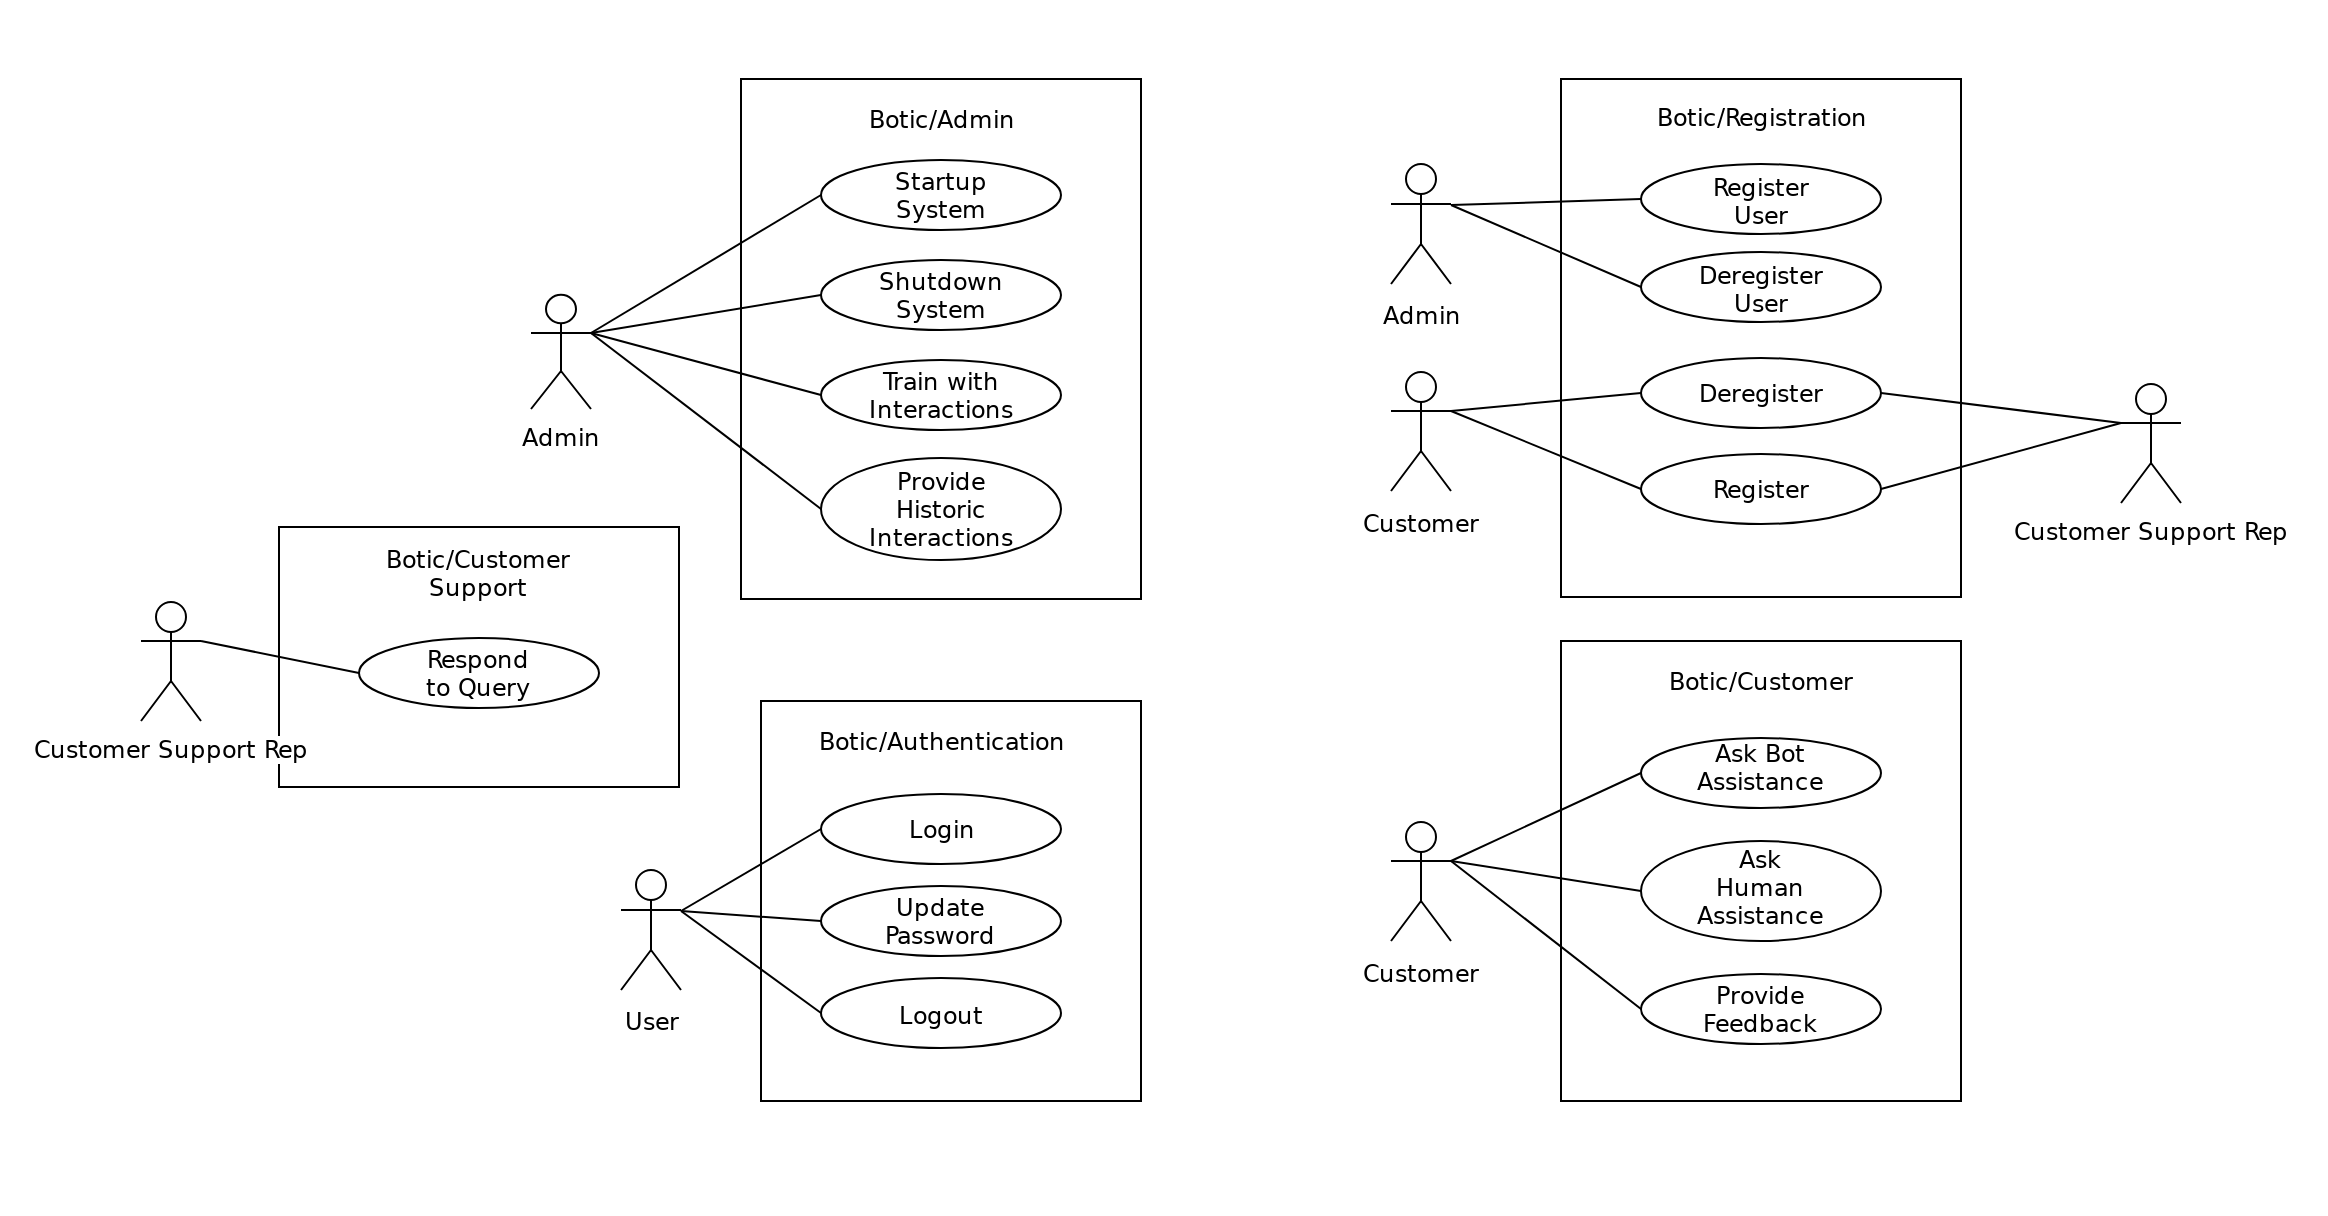
\includegraphics[width=1.2\textwidth]{../../images/Botic_Use_Case_Context_Diagrams.png}
	\caption{Use Case Contexts}
\end{figure}

\subsection{Allocating Use Cases and Subsystems to Iterations}

\subsection{Producing an Architecture Design}
 - Links to relevent documentation
- Special consideration should be made during modeling and analysis to show resources that need protection and entities that access those resources
- Apply security patterns and security design principles to ensure that security requirements are satisfied.
- security test plan to guide the security test process
 
Planning Phase: Succeeded.
 - First meeting with client
 - Use Case-iteration allocation matrix here.

\section{Iterative Phase}
 Interative Phase:
- All artifacts are listed and the changes can be checked out by cross referencing appropriate artifacts.
- Each phase should logically include changes to all the implementation documentation.
- Special consideration should be made during modeling and analysis to show resources that need protection and entities that access those resources
- Practice secure coding to ensure that security principles and security patterns are applied to produce secure code during the implementation phase-- use quality assurance reviewing to make sure of this.
- Also test for security-- test for each quality requirement really; apply static and dynamic security testing. Functional testing, security test
- Domain modeling should identify and capture security related domain concepts and relationships like the roles and resources accessed by the roles as well as related access priviledges
- Design for security and other non functional requirements important during actor-system interaction modeling

\subsection{Phase 1:}
 - Demo 1 happened here.
 - Phase 2 artifacts to be listed here.

\subsubsection{Accomodating Requirements Change}
 
\subsubsection{Domain Modeling}
 
\subsubsection{Actor-System Iteraction Modeling and User Interface Design}
 
\subsubsection{Behavior Modeling and Responsibility Assignment}
 
\subsubsection{Deriving Design Class Diagram}
 
\subsubsection{Test-Driven Development}
 
\subsubsection{Integration}
 
\subsubsection{Deployment}

\subsection{Phase 2:} 
 - Demo 2 happened here
 - Phase 2 artifacts to be listed here.

\subsubsection{Accomodating Requirements Change}
 
\subsubsection{Domain Modeling}
  
\subsubsection{Actor-System Iteraction Modeling and User Interface Design}
  
\subsubsection{Behavior Modeling and Responsibility Assignment}
  
\subsubsection{Deriving Design Class Diagram}
  
\subsubsection{Test-Driven Development}
  
\subsubsection{Integration}
  
\subsubsection{Deployment}

\subsection{Phase 3:}

\subsubsection{Accomodating Requirements Change}
- Another meeting with clients (include proper date).
- Refined the requirements according to proper rules thus we must refine the use cases. Link to the new SRS.
- Updated architectural desgin.
- Link the updated specific requirement and the use cases.
- List of use cases to implementated (before and after)
- No actionable customer feedback

P: Iteration Use Cases
- Haven't produce new ones out of necessity.
- Placing emphasis on the Chatbot component that is meant to use all subsystem.
- Using updated Architecture

\subsubsection{Domain Modeling}
- Domain Model has been updated.

\subsubsection{Actor-System Iteraction Modeling and User Interface Design}

\subsubsection{Behavior Modeling and Responsibility Assignment}

\subsubsection{Deriving Design Class Diagram}

\subsubsection{Test-Driven Development}

\subsubsection{Integration}

\subsubsection{Deployment}

\section{References}
%\bibliographystyle{IEEEtran}
%\bibliography{references}

\end{document}